% !TeX spellcheck = en_GB

\section{Problem 5}

In what follows, we present the development process of our \textbf{near duplicates} search, performed over the recipes corpus we used in homework 1. You can find the source code in the material attached with this documentation.\medskip

\noindent\textbf{Disclaimer}: to run our code, be sure to have Python 2.7 installed. Note that some additional Python modules are required (see following sections).

\subsection{Shingling}

Our first step was to apply \textbf{shingling}\cite{shin} on each document of the corpus to get a \textbf{set representation} that preserves, as much as possible, the \textbf{order} of the words in it. It is crucial when evaluating similarity between two documents.
Indeed, using the simple \textbf{bag of words} model may lead to wrong results. For instance, in these settings, two documents with many terms in common, regarding completely different topics, may be considered similar.
That behaviour has to be avoided, in particular, in cases when similarity search is preparatory to duplicates elimination.\\
Note that we decided to apply shingling \textbf{directly on documents}, rather than on their \textbf{tokens} (as it is often done in practice, for the sake of efficiency). For instance, the string \textit{"a rose is a rose is a rose"} maps to a set of 4-shingles equal to
\begin{center}
\textit{\{' is ', 'rose', 'is a', 'se i', 'ose ', 'a ro', 'e is', ' ros', 's a ', ' a r'\}}
\end{center}
\medskip

\noindent We created a separated Python module (named \textit{shingling.py}) encapsulating the logic of this technique. We also provide a function that returns the \textbf{hashes} of the elements in the set of shingles for a given document, as requested (using the hash family provided in the homework requirements).

\subsection{Brute force approach}

We needed a reference to evaluate the precision of LSH approach (see next section), thus, we made a Python script (named \textit{brute\_force\_near\_duplicates.py}) to explicitly compute the \textbf{Jaccard similarity}\cite{jacc} between each pair of document in the corpus. The output of this script is the set of pairs of documents $(A,B)$ such that $J(A,B) \ge 0.8$ (using their shingles set representation). We say say that such pairs are \textbf{near duplicate} documents.\\
To run the script, open a terminal and type
\begin{lstlisting}
$ python brute_force_near_duplicates.py
\end{lstlisting}
\medskip

\noindent Note that the programs will take much time to terminate (even few hours), since the corpus is quite big (11300 documents) and it has to evaluate similarity for each single pair. We performed some optimizations to reduce running time as much as possible:
\begin{itemize}
\item We avoided comparing a document with itself and evaluating the same pair twice, since $J(A,B) = J(B,A)$ (i.e. we only scan "an half" of the $11300 \times 11300$ matrix).

\item Set union is quite expensive to compute. Therefore, we used
\begin{align*}
J(A,B) = \dfrac{|A \cap B|}{|A \cup B|} = \dfrac{|A \cap B|}{|A|+|B|-|A \cap B|}
\end{align*}
that allows us to only compute intersection.
\end{itemize}

\noindent In addition, since the result of this script is constant, we dumped the resulting set and the related statistics on disk, to easily reuse them when evaluating LSH approach (we used the \textit{pickle}\cite{pickle} module to create a \textit{.pickle} file representing the set of pairs).

\subsection{Minhash and LSH}

Computing Jaccard similarity for each pair of documents is too costly, in particular, for big corpora (a quadratic number of comparisons has to be performed).
Therefore, in practice, we use approximated approaches to get a similar result in much \textbf{less time}.\\
In this case, we used \textbf{Locality-Sensitive Hashing} (LSH)\cite{lsh}, that is a technique whose aim is to maximize the \textbf{probability of collision for similar items}. To do that, it is necessary to have a suitable hash function $h(\cdot)$, that can be obtained applying \textbf{min-wise independent permutations}\cite{minhash} technique (also known as \textbf{minhash}).
Let $A \in \mathcal{X}$ be a document of the corpus, represented as its \textbf{shingles set}. Let $\mathcal{U}$ be a ground set of $m$ elements, such that every possible shingle is included in it. Hence,
\begin{align*}
A = \{a_1, a_2, \ldots, a_k\} \subseteq \mathcal{U} \quad \forall A \in \mathcal{X}
\end{align*}

\noindent Let $r: \mathcal{U} \longrightarrow [1,m]$ be a \textbf{random permutation}. We have
\begin{align}
h(A) = \min_{i \in [1,k]} r(a_i) \quad \forall A \subseteq \mathcal{U} \label{minhash}
\end{align}

\noindent that is the \textbf{minhash signature} of the document.\\
Min-wise hashing satisfies a very nice property: let $A,B$ be any pair of documents in $\mathcal{X}$; we have that collision probability of $A$ and $B$ is directly related to their Jaccard similarity. Indeed,
\begin{align}
\Pr[h(A) = h(B)] = J(A,B) \quad \forall A,B \in \mathcal{X} \label{lsh_prob}
\end{align}

\noindent This \textbf{sketching} scheme is extremely elegant but unfeasible in practice. It would require way too much time and space to actually compute and store the permutations and selecting the minimum element for each set. However, we can give up the idea of using actual random permutations and use \textbf{hash functions} to simulate them, getting \textbf{approximately} min-wise independent permutation.\\
Following the approach suggested in \cite{mmd} (section 3.4.3), we came up with practical implementations of minhash and LSH. We made a separated Python module (called \textit{hashing.py}) that encapsulates the logic and provides us with functions to compute the minhash signature of a shingle set and compute document similarities with LSH approach. The latter consists in:
\begin{enumerate}
\item 
Let $n$ be the number of components of a minhash signature and $t$ be the threshold we want to fix for Jaccard similarity ($t = 0.8$, in our case). 
Choose a number of \textbf{bands} $b$ and a number of \textbf{rows per band} $r$ such that
\begin{align*}
\left\{ 
\begin{aligned}
  &n = b \cdot r\\
  &t \simeq \left(\frac{1}{b}\right)^{\frac{1}{r}}
\end{aligned}
\right.
\end{align*}
Note that $b$ and $r$ can be tuned also taking into account the importance of avoiding \textit{"false negatives"} against the desired speed of the approach. If accuracy is important, then pick $b,r$ that define a $t^* < t$.

\item
For each signature, split it in bands (according to $b,r$) and apply to each band a predefined hash function. In this way, we get $b$ different hash tables such that a bucket contains elements that are considered pair-wise \textbf{candidate} near duplicates. Note that, in this settings, two documents are a candidate pair if they agree in \textbf{at least} a band.

\item
For each hash table, iterate over the buckets. For each bucket, evaluate the similarity of each candidate pair, i.e. compute the actual fraction of components of their signature in which they agree. Let $s$ be this value. Retain all pairs such that $s \ge t$.
\end{enumerate}

\noindent We made a script named \textit{"near\_duplicates.py"} to perform this computation and compare the results with brute force approach. To run the script, open a terminal and type
\begin{lstlisting}
$ python near_duplicates.py
\end{lstlisting}
\medskip

\noindent Note that the computation will take a while to terminate (approximately 20 minutes), but it is \textbf{definitively faster} than brute force. The script will also generate a \textit{"results.txt"} file, reporting some statistics on both the approaches.

\subsection{Conclusions}

\textbf{Disclaimer}: in what follows, we will refer to documents through the id number we assigned to each of them. If you want to deeply understand our results, then you can refer to \textit{"mapping.txt"} file in the attached material and check the actual recipes on \cite{bbc}.\\

\noindent We selected two different pairs of $b,r$ to show how the results change according to the priority we give to accuracy and speed. The following picture shows the two different \textit{"S-curves"} we get.

\begin{center}
	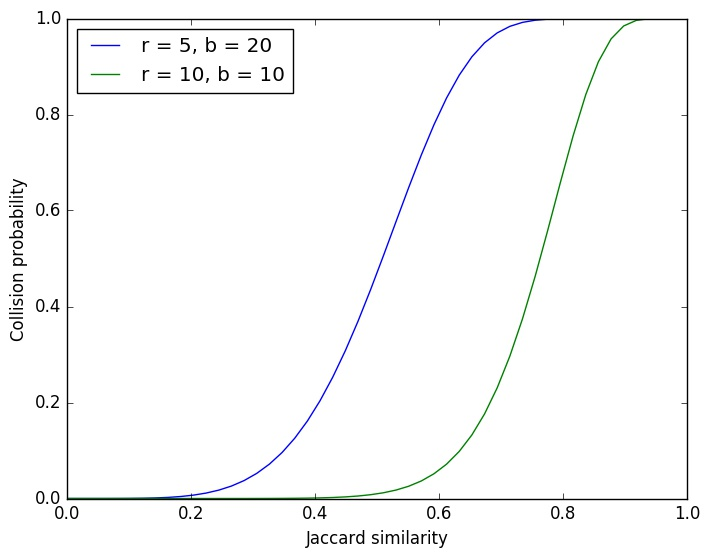
\includegraphics[scale=0.45]{img/lsh_probability.jpg}
\end{center}

\noindent When $r = 10$ and $b = 10$, we have $t^* \simeq t$. As we can see from the plot above, pairs of document with Jaccard similarity equal to $t = 0.8$ have more or less a 0.7 probability to collide (thus, become candidate pairs). Hence, in these settings, LSH would be less accurate (because of the greater probability of having false negatives). The following picture shows an example run.

\begin{center}
	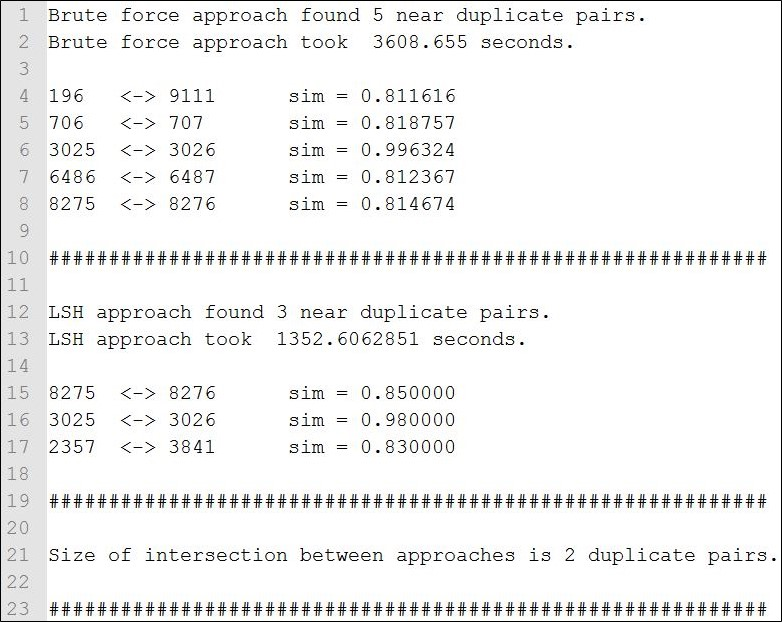
\includegraphics[scale=0.45]{img/results_10_10.jpg}
\end{center}

\noindent On the other hand, when $r = 5$ and $b = 20$, we have $t^* \simeq 0.5 < t$. As we can see from the plot, for Jaccard similarity greater or equal to $t = 0.8$, we are (almost) sure that the collision will occur. Hence, in these settings, LSH would be much more accurate (but obviously slower, because of the greater number of false positives). The following picture shows an example run.

\begin{center}
	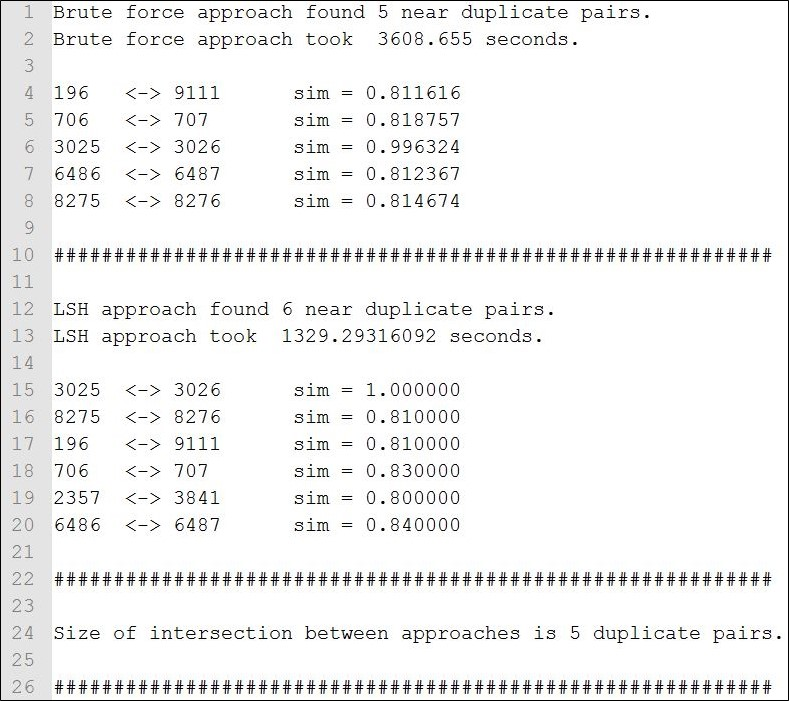
\includegraphics[scale=0.45]{img/results_20_5.jpg}
\end{center}
